\documentclass[a4paper,10pt]{report}
\usepackage[T1]{fontenc}
\usepackage{mathptmx}
\usepackage{graphicx}
\graphicspath{ {Diagrams/} }

\title{Assignment 2.2 documentation}

\author{Péter Zaváczki\\30433}

\begin{document}

\maketitle

\section{Requirements}
Design, implement and test a client-server distributed system that uses RPC to compute taxes
and selling prices for cars. 

\section{Functional requirements}
\begin{itemize}
    \item Users introduce the information of their cars using a simple form (Web or Desktop):
    \begin{itemize}
        \item int year – fabrication year
        \item int engineSize – engine size
        \item double price- purchasing price
    \end{itemize}
    \item The application uses RPC to send the car information to the distributed object from the server that computes the following information depending on the client request:    
    \begin{itemize}
        \item Tax for a car, where the sum depends on the engine size. The equation for calculating the tax, and the sum's variation table can be seen on figure \ref{fig:tax_equation}, respectively figure \ref{fig:tax_sum_variation}.
        
        \begin{figure}[h]
            \centering
            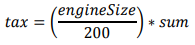
\includegraphics[width=0.25\textwidth]{tax_equation.png}
            \caption{The equation for calculating the tax}
            \label{fig:tax_equation}
        \end{figure}
        
        \begin{figure}[h]
            \centering
            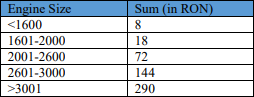
\includegraphics[width=0.5\textwidth]{tax_sum_variation.png}
            \caption{The sum's variation table}
            \label{fig:tax_sum_variation}
        \end{figure}

        \item Selling price for a car, for which you can find the equation on figure \ref{fig:selling_price_equation}.
        
        \begin{figure}[h]
            \centering
            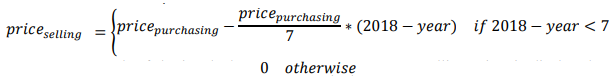
\includegraphics[width=1\textwidth]{selling_price_equation.png}
            \caption{The equation for calculating the selling price}
            \label{fig:s}
        \end{figure}

    \end{itemize}
    \item The result of the invoked operation, tax, respectively selling price, is displayed on the client GUI.
\end{itemize}

\section{Implementation technologies}
\begin{itemize}
    \item Java RMI
    \item Swing
\end{itemize}

\section{Conceptual architecture}
This application has a Client-Server architecture, which uses RPC. The Client being represented by a window containing the user's GUI, and the server, which can serve multiple clients simultaneously.
On the server we bind the implementations of the methods invoked remotely by the client to the RMI register. The RMI register holds the implementations, which the client looks up and uses.
On the client we can find a GUI implemented in Swing, which uses the remote implementations for the ITaxComputationService and ISellingPriceComputationService interfaces.

This can be seen on figure \ref{fig:architecture_diagram}.

\begin{figure}[h]
    \centering
    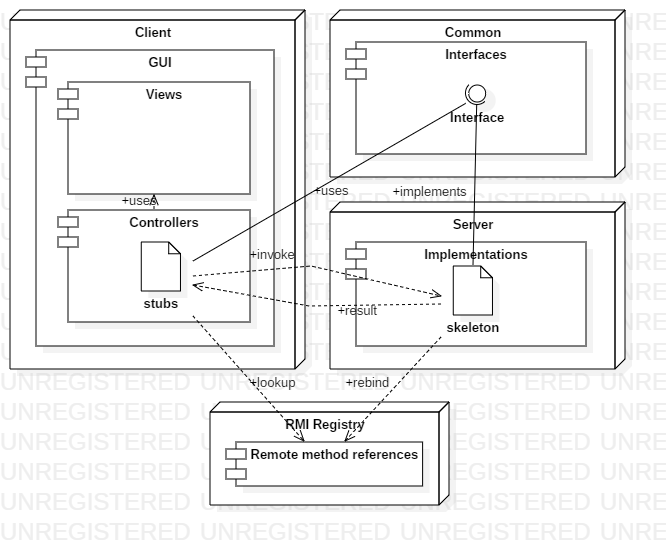
\includegraphics[width=1\textwidth]{architecture_diagram.png}
    \caption{The conceptual architecture diagram of the project}
    \label{fig:architecture_diagram}
\end{figure}

\section{Deployment}
The application is deployed in three parts:
The Client has the application locally, consisting of the GUI, with which he can interact.
The Server has the implementations of the ITaxComputationService and ISellingPriceComputationService interfaces, which are bound to the RMI register.
The RMI register has the references to the implemented remote methods.

This deployment can be seen on figure \ref{fig:deployment_diagram}.

\begin{figure}[h]
    \centering
    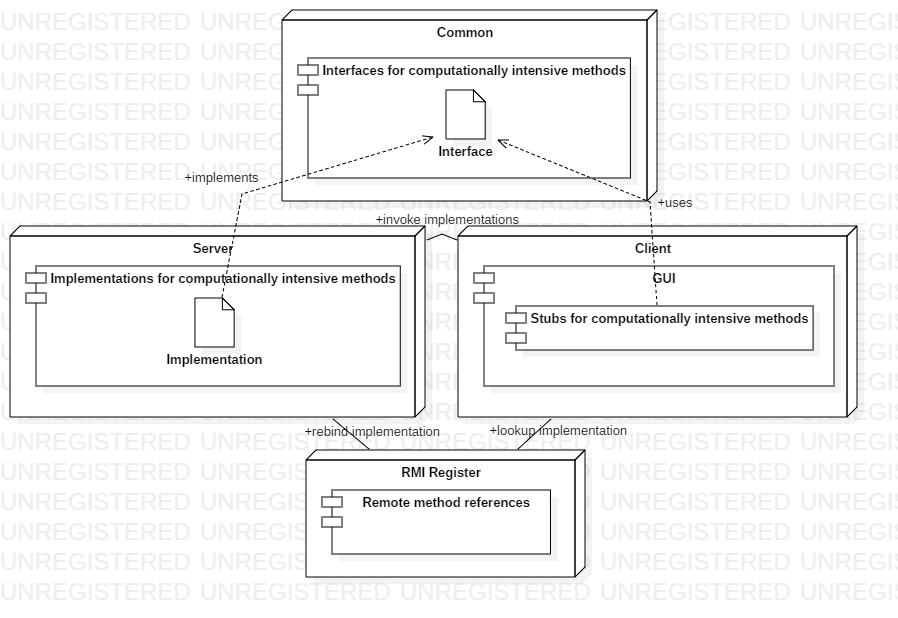
\includegraphics[width=1\textwidth]{deployment_diagram.png}
    \caption{The deployment diagram of the project}
    \label{fig:deployment_diagram}
\end{figure}

\section{Build considerations}
\begin{itemize}
    \item The client's GUI is made in Swing for easier development. As an alternative, a web based GUI could have been made, similarly to the previous assignment.
    \item Java RMI was used instead of .NET Remoting, due to already having knowledge in developing using Java, as opposed to .NET.
\end{itemize}


\end{document}
